\chapter{Uvod}
\label{chp:intro}

\pangrami

\section{Primeri korišćenja klasičnih \LaTeX{} elemenata}
% Primeri citiranja
Ovo je rečenica u kojoj se javlja citat \cite{PetrovicMikic2015}.
Još jedan citat \cite{GuSh:243}.
% Primeri navodnika
Isprobavamo navodnike: "Rekao je da mu se javimo sutra".
% Primer referisanja na tabelu (koja se javlja kasnije)
U tabeli \ref{tbl:rezultati} koja sledi prikazani su rezultati eksperimenta.
% Primer kraćeg ćiriličkog teksta
{\cir Ово је пример ћириличког текста који се јавља у латиничком документу.}
U ovoj rečenici se javlja jedna reč na {\cir ћирилици}.
% Primer korišćenja fusnota
Iza ove rečenice sledi fusnota.\footnote{Ovo je fusnota.}

% Primer dužeg ćirličkog teksta
\begin{cirilica}
  Ово је мало дужи блок текста исписан ћириличким писмом у оквиру
  латиничког документа. Фијуче ветар у шибљу, леди пасаже и куће иза
  њих и гунђа у оџацима.
\end{cirilica}

% Primer korišćenja tabele
\begin{table}
\centering
\caption{Rezultati}
\label{tbl:rezultati}
\begin{tabular}{c>{\centering}p{2cm}c}
\toprule
1 & 2 & 3\\\midrule
4 & 5 & 6\\\cmidrule(rl){1-2}
7 & 8 & 8\\
\bottomrule
\end{tabular}
\end{table}

% Primer korišćenja slike
\begin{figure}[!ht]
  \centering
  \label{fig:grafikon}
  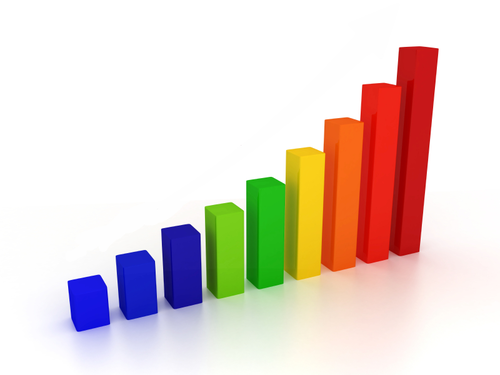
\includegraphics[width=0.5\textwidth]{images/graph.png}
  \caption{Grafikon}
\end{figure}


% Primer jednostavnije matematičke formule
Evo i jedan primer matematičke formule: $e^{i\pi} + 1 = 0$. 
% Primer referisanja na sliku
Na slici \ref{fig:grafikon} prikazan je jedan grafikon.

% primer kompleksnije matematičke formule
$$
\int_a^b f(x)\ \mathrm{d}x \ =_{def}\ \lim_{\max{\Delta x_k \rightarrow 0}} \sum_{k=1}^n f(x_k^*)\Delta x_k
$$

% primer referisanja na poglavlja i strane poglavlja
Više detalja biće dato u glavi \ref{chp:razrada} na strani \pageref{chp:razrada}.

% primer liste
Možemo praviti i nabrajanja:
\begin{enumerate}
\item Analiza 1
\item Linearna algebra
\item Analitička geometrija
\item Osnovi programiranja
\end{enumerate}

\pangrami
